\section{Results}
% Structure with subsections
% Use of figures/tables (max. 5)
% General description of the results
\subsection{Differentially Expressed Genes and Network creation}

Under the chosen thresholds discussed in \ref{sec:methods-deg} 908 genes were found to be differentially expressed. Around half of them (495) are upregulated, the remaining 413 are downregulated. STRING was able to query 828 of them; using other ID types did not change this. After querying the additional EDS-related genes the resulting network consists of 847 nodes and 6129 edges.

The position of the known EDS genes in the network is on average more central than expected by chance based on degree, clustering coefficient, betweenness centralitiy and closeness centrality. This supports the close relationship between hEDS and other EDS types.

\subsection{Enrichment analysis and clustering}

\subsubsection{MCODE}

\begin{itemize}
	\item 3 clusters with more than 15 nodes (first with 66 nodes \& 1953 connections, second with 44 nodes \& 686 connections, third with 16 nodes \& 114 connections)
	\item first and largest cluster upregulated only
	\item second one as well
	\item 3rd MCODE cluster, shown in figure \ref{fig:mcode3}, is mostly upregulated with 2 downregulated nodes, some not relevantly differentially expressed, also only 9/16 are not known eds genes, 8 are
	\item the eds genes are all below the threshold of $|\text{log2FoldChange}| > 0.5$, 1 of them is 1 of the two downregulated genes
	\item quite interesting to see genes closely related to other eds genes, COL21A1 is also strongly upregulated ($\text{log2FoldChange} > 2$)
	\item all known EDS genes with ADAMTS2 as an exception have a high Closeness Centrality
	\item regarding the enrichment of this cluster: not surprising to see the extracellular matrix in two GO-Terms when testing for over-representation of molecular functions
	\item first go term: GO:0005201 - The action of a molecule that contributes to the structural integrity of the extracellular matrix. overall 13 of the 16 genes in this GO-Term, 6 are known eds genes, the other six differentially expressed (COL10A1, COL15A1, PCOLCE, COL5A3, COL18A1, COL21A1, COL27A1)
	\item second go term: GO:0030020 - A constituent of the extracellular matrix that enables the matrix to resist longitudinal stress, and is a subtype of the first. Same EDS genes and same genes as in the first term, except PCOLCE, PCOLE is also the only downregulated gene [TODO: interprete]
\end{itemize}

\begin{figure}[htb!]
	\centering
	\caption*{\textbf{MCODE cluster 3}}
	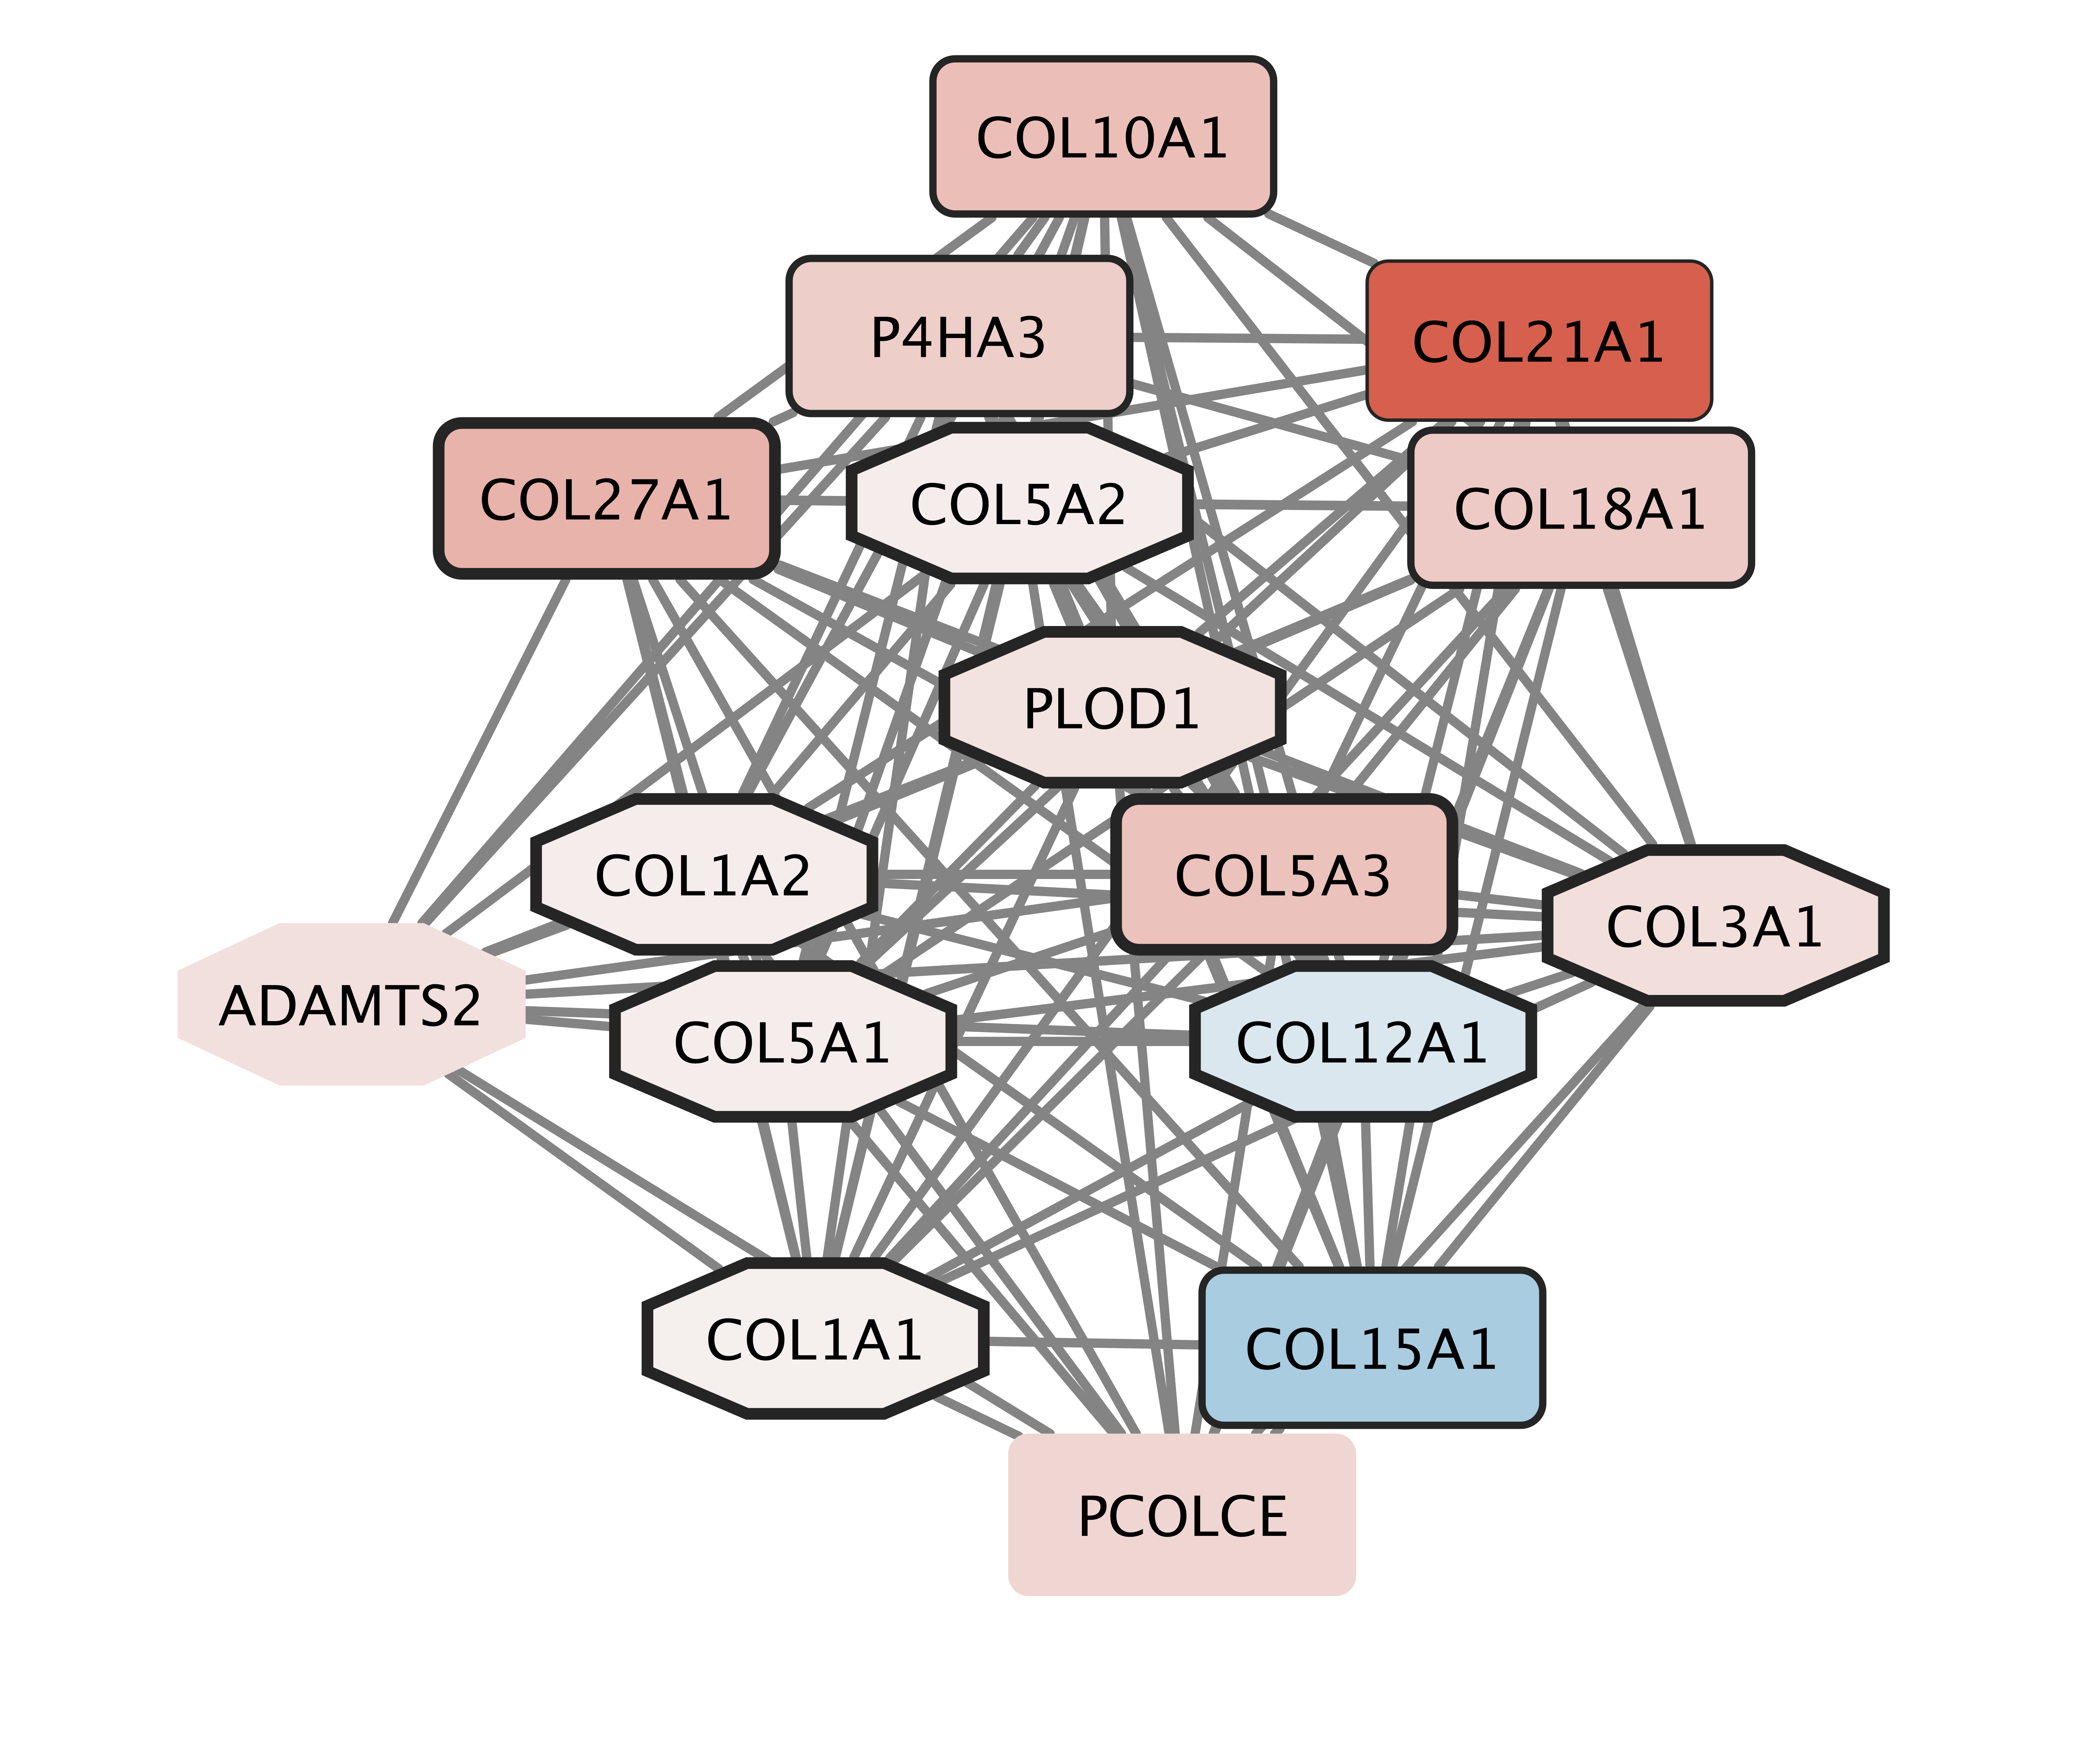
\includegraphics[width=0.6\textwidth]{fig/MCODE-cluster3.png}
	\caption[MCODE cluster 3]{\centering The MCODE cluster contains many genes known to cause other types of EDS. [TODO: add legend for shape and colour]}
	\label{fig:mcode3}
\end{figure}

\begin{itemize}
	\item mcode cluster 2: 	GO:0030527 - structural constituent of chromatin enriched, downregulated genes involved in processes related to chromatin in vEDS \cite{Chiarelli2018}
\end{itemize}

\subsubsection{Community Clustering}

\begin{itemize}
	\item 6 clusters with more than 15 nodes
	\item 3 very small loosely connected clusters (18 nodes \& 17 connections, 29 nodes \& 32 connections, 29 nodes \& 29 connections), two medium-sized highly interconnected (76 nodes \& 1000 connections and 105 nodes \& 2330 connections) and one very large cluster (363 nodes \& 1661 connections)
	\item especially medium-sized clusters highly interconnected
	\item biggest one mix of up-regulated and down-regulated genes, contains all 21 genes known to cause other EDS types
	\item both medium-sized clusters mostly upregulated $\rightarrow$ interesting!
	\item smallest cluster with 18 nodes to small for meaningful enrichment analysis regarding processes
\end{itemize}